\begin{figure*}[t!]
    \centering
    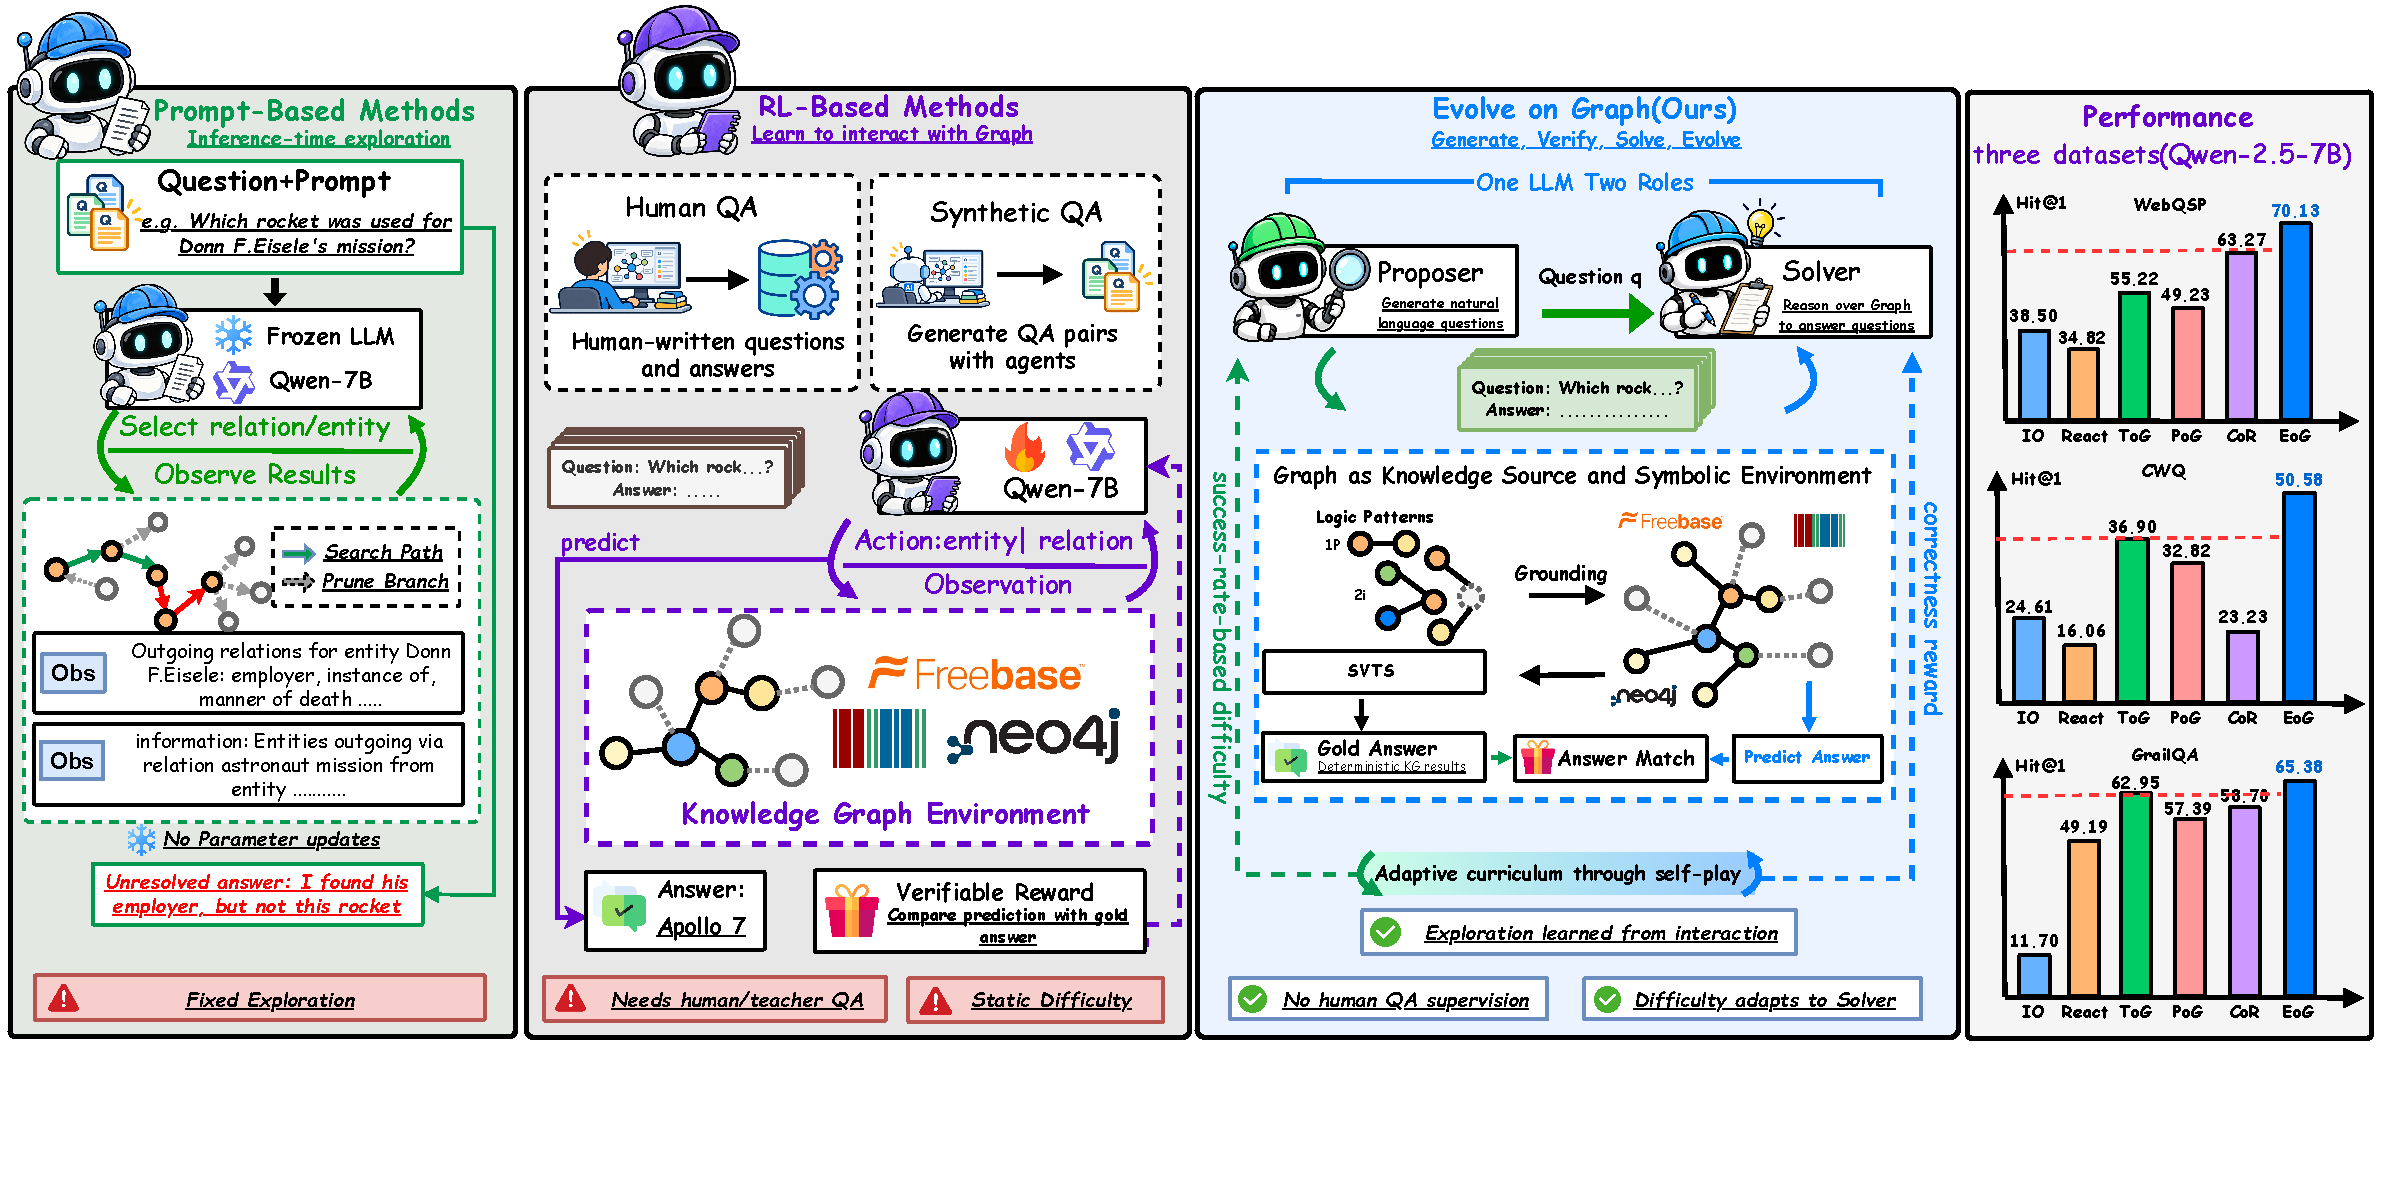
\includegraphics[width=\textwidth]{figures/related_work.pdf}
    \caption{\textbf{Comparison of KG reasoning paradigms.} Prompt-based agents explore with a frozen LLM and RL-based agents learn from fixed QA written by humans or closed-source models, whereas EoG proposes and solves KG-verified tasks of adaptive difficulty. With Qwen-2.5-7B-Instruct, EoG outperforms all shown baselines on three Freebase benchmarks.}
    \label{fig:paradigm}
    \vspace{-5mm}
\end{figure*}
\section{Introduction}
\label{sec:intro}
Large language models (LLMs)~\citep{qwen} have shown remarkable abilities across a wide range of natural language processing tasks~\citep{CoT,Self-Consistency}, yet in complex reasoning that requires deep, multi-hop, and structured factual knowledge, they remain limited by insufficient coverage of long-tail knowledge and by factual hallucinations~\citep{hallucination_1}.

Knowledge graphs (KGs)~\citep{roadmap} store large-scale structured facts and provide reliable external knowledge for LLM reasoning, but this requires the LLM to locate the facts needed at each reasoning step in a large and heterogeneous graph. Research on this problem has moved from one-shot graph retrieval~\citep{RoG,SubGraphRAG,GCR,S-Path-RAG,TARD} toward multi-turn graph exploration (Figure~\ref{fig:paradigm}). Training-free agents~\citep{ToG,PoG,Paths-over-Graph,Open-WorldKG-RAG} prompt a frozen LLM to select relations and entities step by step, while RL-based agents~\citep{KG-R1,GraphWalker,Graph-RFT,ReasoningbyExploration} treat the KG as an interactive environment and train the exploration policy on question--answer data with reinforcement learning (RL). However, most KGs in real-world settings such as industry and healthcare~\citep{KAG,MedRAG} come without any question--answer annotations, and their data often cannot be handed to closed-source models~\citep{PrivGemo}. This raises a question: \emph{can an LLM improve its graph reasoning on a KG using only the KG itself, without any question--answer annotations?}

Answering this question, existing methods still face three challenges. (1) \textbf{The exploration ability of training-free agents cannot improve through interaction.} Training-free agents need no annotations and can be applied to a new KG directly, but their exploration strategy is fixed by the prompt and the frozen backbone, so they cannot accumulate experience from interacting with the graph, and their performance drops sharply on small open-source models~\citep{SLMExploration,RPO-RAG}. (2) \textbf{Training data rely on human annotation or closed-source models.} RL-based agents need large amounts of question--answer data: human annotation~\citep{webqsp,cwq,grailqa,DBLP:conf/nips/ZhangJCCEWWZPWM25,EC-spLLM} requires experts familiar with the KG schema and has to be redone for every new KG, while automatic synthesis~\citep{GraphWalker,GRAIL,GraphScout} relies on closed-source models to synthesize question data. On a KG without annotations that cannot be exposed to closed-source models, neither kind of data is easy to obtain. (3) \textbf{The topology of training tasks cannot follow the agent's ability.} The difficulty of a graph reasoning question lies mainly in its reasoning topology. Existing training data fix the mix of topologies offline before training~\citep{GraphDancer,KnowCoder-A1} and do not adjust it as the agent learns. As the agent grows stronger, simple topologies are already mastered while complex ones remain unsolvable, and neither provides effective learning signals.

To address these challenges, we propose \textbf{Evolve on Graph (EoG)}, a framework in which a single LLM self-evolves on a KG using only the KG itself (Figure~\ref{fig:overview}). First, we propose \textbf{Graph Self-Play}, in which the same LLM alternates between a \emph{Proposer} that poses questions and a \emph{Solver} that answers them. The Proposer explores the graph from real anchor entities, recovers the facts, and writes a question, while the Solver explores the graph to answer it. The two roles share parameters. Second, we propose \textbf{Symbolically Verifiable Topology Synthesis (SVTS)}, which samples reasoning topologies on the graph and executes the corresponding first-order logic queries, giving each task a topology skeleton and a sound and complete answer set. The Proposer explores the graph according to the topology skeleton and writes a multi-hop question. In this way, training tasks and their answers come only from the KG itself, without human annotation or closed-source models. Third, we propose the \textbf{Boundary-Aware Graph Curriculum}, which reinforces the Proposer according to the Solver's score variance, so that it keeps posing questions on the Solver's \emph{capability boundary}, i.e., questions the Solver has not mastered but can still solve. As the Solver grows stronger, more questions on complex topologies fall on its boundary and enter training, forming a graph curriculum that evolves with the Solver.

On six benchmarks over Freebase, Wikidata, and an industrial KG, EoG outperforms prompting-, agent-, and retrieval-based methods without any annotations. With Qwen-2.5-7B-Instruct, EoG exceeds the strongest baseline by +7.46 (Hit@1) and +12.05 (F1) on average, and by +17.80 (Hit@1) on the industrial KG. EoG thus offers a new self-evolving path for training LLM graph reasoning on real-world KGs without any question--answer annotations.
